\chapter{Systèmes linéaires à temps invariant}
\label{chap:lti}
	Le but de ce chapitre est de présenter les concepts de base indispensables à l'étude des systèmes linéaires à temps invariants (LTI) et des signaux.
	Après une définition des critères qui caractérisent un système LTI, nous chercherons à répondre à la question suivante :
	comment déterminer efficacement la réponse d'un système linéaire lorsqu'il est soumis à une excitation quelconque ? Par efficacement, nous entendons :
	\begin{itemize}
		\item méthode mathématiquement "simple"~;
		\item méthode indépendante de l'excitation et des propriétés du système LTI.
	\end{itemize}
	
%	\vspace{1\baselineskip}
	
	Pour cela, nous commencerons par nous interroger sur la manière de représenter l'interaction entre l'entrée et la sortie d'un système, puis sur les notions d'excitation et de réponse. Nous distinguerons les notions de réponses naturelles et forcées, avant d'identifier deux familles d'excitation adaptées à l'étude des systèmes : exponentielle complexe et impulsionnelle. Nous introduirons ensuite la notion de fréquence (complexe), qui nous offrira la possibilité d'étudier les signaux temporels dans le domaine fréquentiel, ainsi que la notion de fonction de transfert qui facilitera l'étude des systèmes.
	
	
	\section{Définition d'un système linéaire à temps invariant}

	\subsection{Linéarité} 
	Un système relie à chaque signal d'entrée $x$ un signal de sortie unique $y$. Les signaux $x$ et $y$ sont des fonctions de la variables réelle appartenant à un espace de fonction le plus général possible noté ici $L_E$. La relation entrée-sortie est donc modélisée par une application mathématique de $L_E$ dans $L_E$ notée $L$ et définie ainsi~:
	\begin{equation}
		L : \application{L_E}{L_E}{x : t\mapsto x(t)}{y : t\mapsto y(t)} 
	%DONE : correction TYPAGE et remarque notation
	\end{equation}

	\begin{remark}{}
	    Remarquons que l'application $L$ transforme une fonction en une fonction et que cela peut compliquer les notations, aussi il est courant de voir utiliser les crochets [] autour des fonctions arguments de l'application $L$ et les simples parenthèses autour de la variable réelle argument d'une fonction. Ce genre d'application est souvent désignée par le terme d'\emph{opérateur}
	    
	    Beaucoup d'abus de notation figurent dans la littérature, gardons à l'esprit et tentons cette année encore de conserver une rigueur d'écriture irréprochable pour garder les idées claires. Parmi les écritures suivantes, une est parfaitement correcte et représente un réel~; une représente correctement une fontion mais ne respecte pas la convention des crochets~;, une est incorrecte~; une est correcte mais lourde à écrire. À vous de les retrouver~:
	    \begin{itemize}
	        \item $y(t) = L[x(t)]$~;
	        \item $y = L(x)$~;
	        \item $y(t) = L[x](t)$~;
	        \item $t\mapsto y(t) = L[t\mapsto x(t)]$
	    \end{itemize}{}
	\end{remark}
	
	Une classe de système fondamentale est la classe des systèmes linéaires car elle offre de nombreux outils et propriétés mathématiques.
	\begin{definition}{Système linéaire}
	\label{def:linearite}
	Une système est dit linéaire si et seulement si l'application $L$ associée est linéaire, soit
	pour tout $\p{x_1,x_2,y_1,y_2,\lambda} \in L_E^4 \times \R$~:
	\begin{eqnarray}
    	\label{eq:def_linearite}
	    \forall t \in \R \qquad L\b{x_1 + \lambda\, x_2}(t) = y_1(t) + \lambda\,y_2(t) \nonumber\\
	    \text{ou bien } \qquad L\b{x_1 + \lambda\,x_2} = x_1 +\lambda L\b{x_2 }
	\end{eqnarray}
	\end{definition}
	

	Une des conséquences de la linéarité est la possibilité d'appliquer le principe de superposition.
	
	%TODO on va considérer d'autres systèmes ! j'enlèverai cette partie qui n'amène pas grand chose...
	Les trois opérateurs linéaires de base que nous considérons dans l'étude des systèmes linéaires sont :
	\begin{itemize}
		\item proportionnel : $y = a\cdot x$ où a est une constante 
		\item intégration : $y = a\cdot \int f(x) \deriv x $ où a est une constante
		\item dérivée : $y = a\cdot \frac{df(x)}{dx} $ où a est une constante
	\end{itemize}
	On peut aisément vérifier qu'il respecte la condition \ref{eq:def_linearite}.
	%Fin du todo
	
	
	\subsection{Invariance temporelle}
	%DONE rédaction en définition
	Il est fréquent qu'un système réagisse de la même manière indépendemment de l'instant où est appliqué le signal d'entrée. Ce qui conduit à la définition suivante~: 
	\begin{definition}{Système invariant dans le temps}
	Un système est dit invariant dans le temps si et seulement si son application associée $L$ vérifie~:
	\begin{equation}
	\forall t\in \R, \; L[t\mapsto x(t-t_{0})] = L[x](t-t_{0}) 
	\end{equation}
	\end{definition}
	
	En d'autres termes, la réponse du système ne dépend pas de l'origine des temps choisie.
	
	\begin{example}
	%TODODONE typage !!!
	L'effet d'un système sur le signal d'entrée est d'écrit par l'application : $x \mapsto y=2\frac{dx}{dt}$.
	Vérifions d'abord que cet opérateur est linéaire~:
	Soit $ \p{x_1,x_2,y1,y2}\in L_E^4$ telles que $L\b{x_1}=y_1$ et de même pour $x_2$ et $y_2$. Vérifions que pour toute entrée $x_{3} : t\mapsto x_{1}(t)+\lambda\,x_{2}(t) $ avec $\lambda\in\R$ on ait  :
	\begin{eqnarray*}
	L\b{x_1+\lambda x_2} = t \mapsto 2\frac{d}{dt}\p{x_1+\lambda x_2}
	y_{3}(t)=2a\frac{dx_{1}}{dt}+2b\frac{dx_{2}}{dt}
	y_{3}(t)=ay_{1}(t)+by_{2}(t)
	\end{eqnarray*}
	Le système est donc linéaire. Vérifions son invariance temporelle :
	\begin{equation*}
	x(t-t_{0}) \rightarrow 2\frac{d}{dt}x(t-t_{0})=y(t-t_{0})
	\end{equation*}
	\end{example}
	
	
	\subsection{Passivité}
	Dans ce cours, on considèrera aussi des systèmes passifs, dans le sens où il n'y a pas d'énergie emmagasinée ou fournie par une entrée autre que celle sur laquelle on applique le signal d'entrée étudié.
	\subsection{Causalité}
	L'étude des systèmes linéaires passent par l'étude et la synthèse de fonctions mathématiques. Tous les systèmes linéaires physiquement réalisables peuvent être décrits par une fonction mathématique linéaire. Par contre, la réciproque n'est pas forcément vraie : un système décrit par une fonction linéaire n'est pas nécessairement physiquement réalisable. Une caractéristique importante qui différencie les systèmes physiquement réalisables de ceux qui ne le sont pas est la notion de causalité. On entend par physiquement réalisable un système pouvant traiter en temps réel les signaux d'entrée.
	Dans un système causal, l'effet ne peut pas précéder la cause (\ref{def_causal}). Un système sera physiquement réalisable s'il est causal, c'est-à-dire que sa réponse ne dépend que des états présents et passés de l'excitation.
	
	\begin{equation}\label{def_causal}
	\forall t < t_{0} : x(t) = 0 \rightarrow \forall t < t_{0} : y(t) = 0
	\end{equation}
	
	Les systèmes numériques peuvent être non causaux car ils sont capables de stocker les valeurs du signal d'entrée pour un traitement différé. On peut prendre l'exemple de l'application de floutage d'une image numérique. Celle-ci correspond à une matrice de données, représentant chaque pixel de l'image. Le floutage consiste à appliquer un filtre (par exemple gaussien) qui sera centré sur chaque pixel. Ce filtre effectue une somme pondérée du pixel central mais aussi des pixels voisins, situés avant et après le pixel central. L'effet du floutage d'un pixel dépend donc de pixels situés après dans l'ordre de rangement des pixels. 

	
	
	\section{Equation générale d'un système linéaire}
	La réponse d'un système linéaire sera gouvernée par trois types d'effet, pouvant se superposer : proportionnel, différenciateur et intégrateur. Globalement, un système linéaire est gouverné par une équation différentielle ordinaire donnée par \ref{equation_generale_LTI}. On l'appelle l'équation générale du système. Pour une excitation x(t) donnée, sa résolution permettra de déterminer la réponse y(t).
	
	\begin{equation}\label{equation_generale_LTI}
	\sum_{i=0}^M a_{i}\times \frac{d^{i}y}{dt^{i}} = \sum_{j=0}^N b_{j}\times \frac{d^{j}x}{dt^{j}}
	\end{equation}
	
	
	\section{Réponse d'un système}
	La réponse d'un système correspond au signal (ou aux signaux) de sortie lorsqu'il est excité par un (ou plusieurs) signal d'entrée. En reprenant l'équation générale \ref{equation_generale_LTI}, on remarque que l'on peut distinguer :
	\begin{itemize}
		\item la réponse propre ou naturelle d'un système, notée $y_{0}(t)$, correspondant à la solution de l'équation différentielle pour une excitation nulle.
		\item la réponse forcée, notée $y_{f}(t)$ correspondant à la solution de l'équation différentielle pour une excitation particulière x(t).
	\end{itemize}
	
	La réponse d'un système sera la superposition de ces deux réponses.
	
	\begin{equation}
	y(t) = y_{0}(t)+y_{f}(t)
	\end{equation}
	
	Dans la suite du cours, nous ne nous intéresserons qu'à des systèmes causaux,  et nous considérerons que les excitations sont nulles pour t < 0.
	
	\section{Réponse naturelle d'un système LTI}
	Il s'agit de la partie de la réponse qui est indépendante de l'excitation. Elle est donc intrinsèque aux caractéristiques du système. Elle se détermine en résolvant l'équation différentielle \ref{equation_generale_LTI} dans le cas où l'excitation x(t) est nulle.
	\begin{equation}\label{equa_diff_reponse_naturelle}
	\sum_{i=0}^M a_{i}\times \frac{d^{i}y}{dt^{i}} = 0
	\end{equation}
	On pourrait s'interroger sur le sens de cette réponse. Si le système n'avait pas emmagasiné d'énergie au départ, la réponse serait nulle, ce qui ne présente pas d'intérêt pour l'étude des systèmes. La réponse naturelle n'apparait que si le système a été préalablement excité avant t = 0.  
	
	Comme l'excitation disparait pour t > 0, la réponse sera forcément transitoire. Seule une fonction présentant la même forme avant/après dérivation plusieurs fois peut être solution de l'équation \ref{equa_diff_reponse_naturelle}. Il n'existe qu'une seule forme de fonction avec une telle propriété : la forme exponentielle complexe donnée par (\ref{expo_complexe}).
	\begin{equation}\label{expo_complexe}
	y_{0}(t) = A \cdot exp(p t)       
	\end{equation}
	avec A et p $\in \mathbb{C}$. La forme générale de la réponse naturelle sera donc donnée par $ \sum_{i=0}^M a_{i}\cdot p^{i} \cdot exp(p \cdot t) $. Hormis la solution triviale $y_{0}(t) = 0$, la solution ce cette équation est donnée par \ref{solution_reponse_naturelle}.
	\begin{equation} \label{solution_reponse_naturelle}
	\sum_{i=0}^M a_{i}\cdot p^{i} = 0 \Rightarrow \prod_{i=1}^{M} (p-p_{i}) = 0     
	\end{equation}	
	Ce polynôme est appelée l'équation caractéristique du système. En effet, les caractéristiques de la réponse naturelle du système sont liées aux M solutions ou racines $p_{i}$ de cette équation. La réponse naturelle peut alors s'écrire sous la forme suivante :
	\begin{equation}\label{reponse_naturelle}
	y_{0}(t) = \sum_{i=1}^M A_{i}\cdot exp(p_{i} \cdot t) 
	\end{equation}
	où les termes $A_{i}$ dépendent des conditions initiales connues en un temps $ t_{0}$.
	
	\vspace{1\baselineskip}
	
	\subsection{Fréquences naturelles d'un système LTI}
	Les M racines de l'équation caractéristique du systèmes sont appelées les fréquences naturelles ou fréquences propres du système. Elles sont complexes et de la forme suivante :
	\begin{equation}\label{freq_propre}
	p_{i} = \sigma_{i} + j\omega_{i} 
	\end{equation}	
	En reprenant \ref{reponse_naturelle}, la réponse naturelle pourra s'exprimer en fonction de ces fréquences naturelles :
		
	\begin{equation}\label{Reponse_Naturelle}
	y_{0}(t) = \sum_{i=1}^M A_{i}exp(\sigma_{i}  t) exp(j\omega_{i} t)
	\end{equation}
	$\omega_{i}$ caractérise la pulsation de la réponse associée à cette racine, tandis que la partie réelle $\sigma_{i}$ indique l'atténuation ou l'amortissement de cette réponse. Leur connaissance est indispensable car ce sont elles qui caractérisent la forme temporelle de la réponse du système. La prédiction de l'évolution temporelle de la réponse du système va passer par l'analyse de ces racines. 
	
	\subsection{Plan p}
	Puisque les racines de l'équation caractéristique déterminent la réponse naturelle d'un système, il est intéressant d'établir un système de représentation graphique facilitant l'analyse du système. C'est le but de la représentation appelée plan complexe ou plan P , illustré à la figure \ref{Fig:Plan_P}. Il s'agit d'un repère cartésien dans lequel les racines sont placées, permettant de visualiser leurs parties réelles et imaginaires. Selon le positionnement des racines dans le plan P, les caractéristiques du système seront différentes, notamment sa stabilité.
	\begin{figure}[h!]
		\centering
		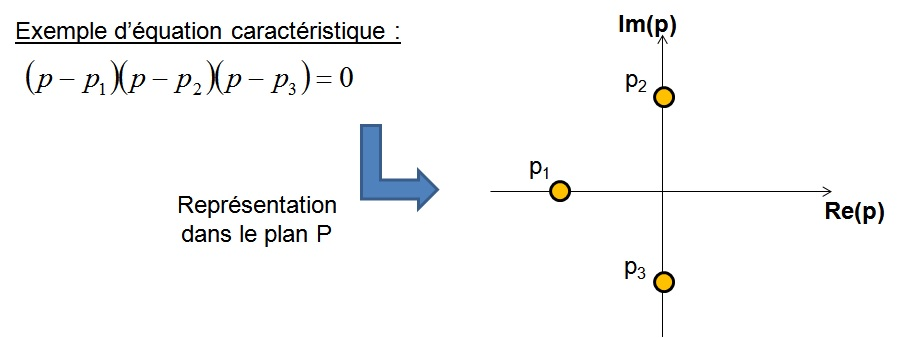
\includegraphics[scale=0.5]{images/Plan_P.jpg} 
		\caption{Placement des racines de l'équation caractéristique dans le plan P}	
		\label{Fig:Plan_P}
	\end{figure}

	\subsection{Analyse du plan p - Stabilité du système}
	La stabilité d'un système est une notion qui sera abordée plus en détail dans les cours d'automatique. Dans ce cours, nous utiliserons une définition au sens large : on entend par stabilité le fait que la réponse d'un système converge vers une valeur finie quelle que soit l'excitation appliquée (à condition que cette excitation converge). Dès que l'on conçoit un système, c'est une propriété indispensable qui doit être vérifiée.
	Un système est stable si et seulement si à toute entrée bornée, il fait correspondre une sortie bornée :
	\begin{equation}
	(\forall t \in \mathbb{R})~(|x(t)| \leq A),~avec~A \in \mathbb{R} \Rightarrow (|y(t)| \leq B),~avec~B \in \mathbb{R}
	\end{equation}
	
	
	La position des racines de l'équation caractéristique détermine à la fois la stabilité du système linéaire, mais aussi la forme temporelle de réponse. Pour l'admettre, considérons les cinq cas suivants, correspondant à cinq positions différentes d'une racine $p_{i}$ dans le plan P, et déterminons le type de réponse temporelle. On considère t > 0 :
	
	
	\begin{enumerate}
		\item $p_{i}$ est purement complexe ($\sigma_{i}$ = 0) : elle est située sur l'axe des ordonnées du plan P. La réponse  naturelle sera donc un signal purement (co)sinusoïdale, dont l'oscillation aura une fréquence ou une pulsation déterminée par $\omega_{i}$. Le système est en limite de stabilité car sa réponse oscille en permanence autour d'une valeur.
		\item $p_{i}$ est purement réel et négatif ($ \sigma $\textsubscript{i} \textless{} 0 et 		$ \omega $\textsubscript{i} = 0) : la racine est située sur l'axe des abscisses à 		gauche de l'origine. La réponse est une fonction exponentielle 		décroissante, sans la moindre oscillation, indiquant un comportement	amorti. La réponse naturelle indique un système parfaitement stable.
		\item $p_{i}$ est purement réel et positif ($ \sigma $\textsubscript{i} \textgreater{} 0 et $ \omega $\textsubscript{i} = 0) : la racine est située sur l'axe des abscisses à droite de l'origine. La réponse est une fonction exponentielle croissante, sans la moindre oscillation, indiquant un comportement divergeant. La réponse naturelle indique un système instable.
		\item $p_{i}$ est une valeur complexe quelconque dont la partie réelle est négative ($ \sigma $\textsubscript{i} \textless{} 0 et  $ \sigma_{i} \neq 0 $) : la racine 	est située dans le demi plan à gauche de l'axe es ordonnées. La réponse va présenter une oscillation dont la fréquence est déterminée par $ \omega_{i}$, mais dans l'amplitude s'atténue plus ou moins rapidement au cours du temps selon la valeur  $ \sigma_{i} $. Cette réponse indique un système stable.
		\item $p_{i}$ est une valeur complexe quelconque dont la partie réelle est positive ($ \sigma $\textsubscript{i} \textgreater{} 0 et $ \omega_{i} \neq 0 $) : la racine est située dans le demi plan à droite de l'axe es ordonnées. La réponse va présenter une oscillation dont la fréquence est déterminée par $ \omega_{i} $, mais dans l'amplitude s'accroit plus ou moins rapidement au cours du temps selon la valeur  $ \sigma_{i} $. Cette réponse indique	un système instable.
		

	\end{enumerate}
	
	La figure ci-dessous illustre les types de réponse naturelle associées à une fréquence naturelle, selon sa position dans le plan P.
	\begin{figure}[h!]
		\centering
		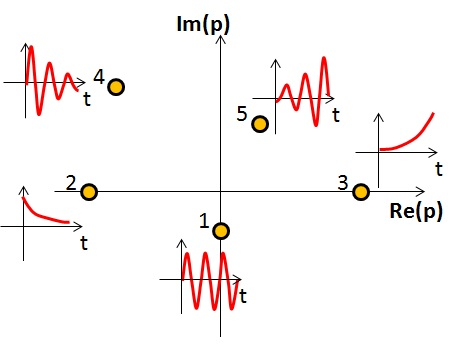
\includegraphics[scale=0.5]{images/reponse_vs_p.jpg} 
		\caption{Types de réponse naturelle en fonction de la position d'une racine dans le plan P.}	
		\label{Fig:reponse_vs_p}
	\end{figure}
	
	\textbf{\underline{Domaine fréquentiel}}
	
	On remarque que l'on est capable de représenter avec un point dans le
	plan p une fonction temporelle de type exponentielle complexe. Il s'agit de la même fonction, mais vue
	dans un autre domaine, que l'on appelle domaine fréquentiel. Dans ce domaine, la fonction n'est plus caractérisée par le temps, mais par sa fréquence. De manière générale, les fréquences sont des grandeurs complexes. Néanmoins, dans le cas de l'analyse des signaux, on ne considère que des fréquences réelles.
	
	
	\subsection{Ordre d'un système linéaire}
	
	Plus l'équation caractéristique présente de racines, plus sa réponse
	devient complexe, puisqu'elle résulte de la superposition de plusieurs
	fréquences  comme le montre l'équation \ref{Reponse_Naturelle}. On appelle l'ordre
	d'un système le nombre de racines que présente son équation
	caractéristique. Il s'agit aussi de l'ordre ou du degré de l'équation
	différentielle caractérisant le système. Pour illustrer la notion
	d'ordre, nous allons analyser la réponse naturelle de deux circuits
	électriques passifs, caractérisés par des équations caractéristiques d'ordre 1 et 2. Vous retrouverez une analyse plus détaillée dans le cours d'électronique.
	
	\subsubsection{Exemple 1 : circuit RC}
		
	\begin{minipage}[l]{0.7\linewidth}
		On considère le circuit ci-contre, formé par une résistance R et un condensateur C. En t = 0, le condensateur est chargé, de sorte que la tension à ses bornes soit égale à $U_{C0}$. On note $U_{C}$ et $U_{R}$ les tensions aux bornes du condensateur et de la résistance. 	
	\end{minipage} \hfill
	\begin{minipage}[r]{0.4\linewidth}
		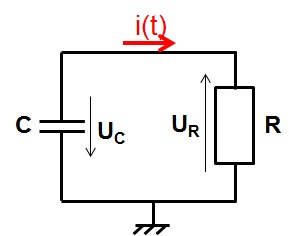
\includegraphics[scale=0.5]{images/circuit_RC_reponse_naturelle.jpg} 	
	\end{minipage}
	\vspace{0.5\baselineskip}
	On souhaite déterminer la réponse naturelle de ce circuit pour t > 0, sous la forme du courant électrique i(t) circulant au travers du circuit. On souhaite aussi déterminer la fréquence naturelle de ce circuit, caractérisant sa réponse transitoire.
	
	\vspace{1\baselineskip}
	Commençons par appliquer la loi des mailles à ce circuit, qui permet d'écrire : $U_{R}(t)+U_{C}(t)=0.$ En prenant en compte les relations tension-courant pour la résistance et le condensateur, cette relation peut être mise sous la forme ci-dessous ne faisant apparaître que le courant. Après différenciation de l'équation, on fait apparaître une équation différentielle du premier ordre. On constate que le terme RC est homogène à un temps. On l'appelle la constante de temps du circuit RC, généralement notée $\tau$.
	\begin{equation*}
	Ri(t)+\frac{1}{C}\int i(t) \deriv t=0~\rightarrow ~\frac{di}{dt}+\frac{1}{RC}i = 0
	\end{equation*}
	On retrouve une équation du même type que \ref{equa_diff_reponse_naturelle}. La solution de cette équation peut donc s'écrire : $i(t) = Ae^{pt}$, où A est lié aux conditions initiales et p est l'unique fréquence naturelle du système. En intégrant cette solution dans l'équation différentielle, on en déduit l'équation caractéristique de ce circuit (\ref{equa_carac_RC}).
	\begin{equation*}
	Ap\cdot e^{pt}+\frac{1}{RC} e^{pt}=0
	\end{equation*}
	\begin{equation}\label{equa_carac_RC}
	p+\frac{1}{RC}=p-p_{0}=0
	\end{equation}
	Cette équation présente une seule racine $p_{0} = -\frac{1}{RC}$. Ce circuit électrique est donc un système d'ordre 1. La racine est purement réelle et négative. Elle se situe donc à gauche de l'axe des imaginaires dans le plan P, traduisant le comportement stable et non oscillant du système (équivalent au point 2 de la figure \ref{Fig:reponse_vs_p}). La fréquence naturelle	indique donc une réponse naturelle du type exponentielle décroissante. Cela est confirmé par l'expression de la réponse naturelle du circuit, qui s'écrit :
	\begin{equation}\label{Reponse_naturelle_RC}
	i(t)=Aexp(p_{0}t)=Aexp(-\frac{t}{RC})~,~~t>0
	\end{equation}
	La valeur de A peut être déterminée à partir des conditions initiales en t = $0^{+}$. Le courant dans le circuit est alors donné par : $i(0)=\frac{U_{R}(0)}{R}=\frac{U_{C0}}{R}$. A partir de \ref{Reponse_naturelle_RC}, on en déduit $A=\frac{U_{C0}}{R}$.


	\subsubsection{Exemple 2 : circuit RLC}
	
	\begin{minipage}[l]{0.7\linewidth}
		On considère le circuit ci-contre, formée par une résistance R, un condensateur C et une bobine L montées en parallèle (R, L et C $\geq$ 0). En t= 0, le condensateur est chargé, de sorte que la tension à ses bornes soit égale à $U_{C0}$. On note $i_{C}$, $i_{R}$ et $i_{L}$ les courants traversant ces trois composants. 	
	\end{minipage} \hfill
	\begin{minipage}[r]{0.4\linewidth}
		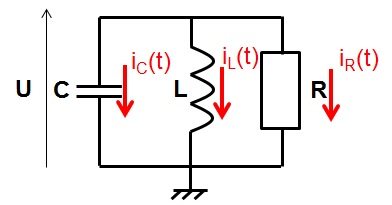
\includegraphics[scale=0.5]{images/circuit_RLC_reponse_naturelle.jpg} 	
	\end{minipage}
	\vspace{0.5\baselineskip}
	On souhaite déterminer la réponse naturelle de ce circuit pour t > 0, sous la forme de la tension u(t) mesurée aux bornes du circuit. On souhaite aussi déterminer la fréquence naturelle de ce circuit, caractérisant sa réponse transitoire.

	\vspace{1\baselineskip}
	Commençons par appliquer la loi des nœuds à ce circuit, qui permet d'écrire : $i_{C}(t)+i_{R}(t)+i_{L}(t)=0.$ En prenant en compte les relations tension-courant pour la résistance et le condensateur, cette relation peut être mise sous la forme ci-dessous ne faisant apparaître que le courant. Après différenciation de l'équation, on fait apparaître une équation différentielle du second ordre. Pour simplifier les notations, on pose : $\alpha = \frac{1}{2RC} $ et $\omega^{2} = \frac{1}{LC}$.
	\begin{equation*}
	C\frac{du}{dt}+\frac{u(t)}{R}+\frac{1}{L}\int u(t) \deriv t=0~\rightarrow ~\frac{d^{2}u}{dt^{2}}+\frac{1}{RC}\frac{du}{dt}+\frac{1}{LC}u(t) = 0
	\end{equation*}
	\begin{equation*}
	\frac{d^{2}u}{dt^{2}}+2\alpha \frac{du}{dt}+\omega^{2}u(t) = 0
	\end{equation*}
	
	On retrouve une équation du même type que \ref{equa_diff_reponse_naturelle}. La solution de cette équation peut donc s'écrire : $u(t) = Ae^{pt}$. En intégrant cette solution dans l'équation différentielle, on en déduit l'équation caractéristique de ce circuit (\ref{equa_carac_RLC}).
	\begin{equation*}
	(p^{2}+2\alpha p+\omega^{2})Ae^{pt}=0 
	\end{equation*}
	\begin{equation}\label{equa_carac_RLC}
	p^{2}+2\alpha p+\omega^{2}=(p+p_{1})(p+p_{2})=0
	\end{equation}
	Cette équation présente deux racines $p_{1}$ et $p_{2}$. Ce circuit électrique est donc un système d'ordre 2, dont la réponse naturelle va s'écrire :
	\begin{equation}\label{key}
	u(t) = A_{1}e^{p_{1}t}+A_{2}e^{p_{2}t}
	\end{equation}
	
	 où $A_{1}$ et $A_{2}$ dépendent des conditions initiales. Selon la valeur de R, L et C, la nature et la position de ces racines dans le plan P va changer, modifiant le comportement transitoire du circuit. Pour déterminer ces racines, il suffit de résoudre une équation d'ordre 2, dont le déterminant est donné par : $\Delta = 4(\alpha^{2}-\omega^{2})$. La nature des racines varie selon le signe du déterminant :
	\begin{equation}
	si~\alpha \geq \omega : \left \{
		\begin{array}{l}
			p_{1}=\frac{-2\alpha +\sqrt{\Delta}}{2}=-\alpha+\sqrt{\alpha^{2}-\omega^{2}} \\
			p_{2}=\frac{-2\alpha -\sqrt{\Delta}}{2}=-\alpha-\sqrt{\alpha^{2}-\omega^{2}} \\
		\end{array}
	\right.
	\end{equation}
	\begin{equation}
	si~\alpha < \omega : \left \{
	\begin{array}{l}
	p_{1}=\frac{-2\alpha +j\sqrt{-\Delta}}{2}=-\alpha+j\sqrt{\omega^{2}-\alpha^{2}} \\
	p_{2}=\frac{-2\alpha -j\sqrt{-\Delta}}{2}=-\alpha-j\sqrt{\omega^{2}-\alpha^{2}} \\
	\end{array}
	\right.
	\end{equation}
	On peut distinguer plusieurs types de comportement transitoire distincts selon les valeurs de $\alpha$ et $\omega$ :
	\begin{itemize}
		\item si $\alpha \neq 0$, alors les deux racines présentent une partie réelle négative. Le système présente donc un caractère stable.
		\item si $\alpha \geq \omega$, les deux racines sont purement réelles et négatives. Dans le plan P, elles sont situées sur l'axe des réels à gauche de l'axe des imaginaires. La réponse du circuit sera du type exponentiel décroissant sans oscillation (équivalent au point 2 de la figure \ref{Fig:reponse_vs_p}).
		\item si $\alpha < \omega$ et $\alpha \neq 0$, les deux racines sont conjuguées. Elles sont situées à gauche de l'axe des imaginaires dans le plan P. La réponse du circuit sera du type oscillation amortie de pulsation $\sqrt{\omega^{2}-\alpha^{2}}$ (équivalent au point 4 de la figure \ref{Fig:reponse_vs_p}). 
		\item si $\alpha = 0$, les deux racines sont purement imaginaires et conjuguées. Elles sont placées sur l'axe imaginaire du plan P, symétriquement à l'axe de réels. La réponse du circuit sera une oscillation non amortie de pulsation $\omega$ (équivalent au point 1 de la figure \ref{Fig:reponse_vs_p}). 
	\end{itemize}
	\vspace{1\baselineskip}

	
	\section{Réponse forcée}
	
	La réponse forcée est la solution de l'équation générale du système pour une excitation non nulle. La réponse va dépendre de la forme de l'excitation, mais aussi des
	propriétés du système. Puisque la réponse dépend de l'excitation, il est
	préférable de déterminer des excitations dont les propriétés
	faciliteront l'analyse de la réponse forcée d'un système. Pour cela, il
	faut chercher des familles d'excitation dont la forme n'est pas modifiée
	par l'effet du système LTI. Ainsi, en connaissant la forme de
	l'excitation, on déduira immédiatement la forme de la réponse. Seuls
	quelques coefficients que nous préciserons seront à calculer.
	
	Nous allons nous intéresser à deux familles d'excitations répondant à ce critère : l'excitation
	exponentielle complexe (que nous avons rencontré précédemment) et la
	famille d'excitation impulsionnelle.
	
	\subsection{Excitation exponentielle complexe}
	L'excitation exponentielle complexe présente la forme suivante :
	
	\begin{equation}\label{exc_expo_complexe}
		x =    \left \{
		\begin{array}{l l}
		\hat{X} \cdot exp(p_{x}t)  & si~t>0 \\
		0   & sinon \\
		\end{array}
		\right .
	\end{equation}
	
	où $ \hat{X} = |X| \cdot exp(j \theta)$ est l'amplitude complexe ou vecteur de Fresnel le phaseur du signal et $ p_{x} = \alpha $+j$ \omega $ sa fréquence complexe. Dans le cas où l'on s'intéresse à des signaux réels (cas rencontré en pratique), cette forme reste valable à condition de ne conserver que la partie réelle. Elle s'écrit alors :
	\begin{equation}\label{exc_expo_complexe_reel}
	x(t) =    \left \{
	\begin{array}{l l}
	Re[\hat{X} \cdot e^{p_{x}t)}] = |X| \cdot e^{\alpha t} \cdot cos(\omega t+\theta)  & si~t>0 \\
	0   & sinon \\
	\end{array}
	\right .
	\end{equation}
	Comme dans le cas de la fréquence naturelle, la fréquence complexe peut
	être représentée dans le plan P. Sa position indique qualitativement la
	forme temporelle de l'excitation. Si p\textsubscript{x} est purement
	réelle, l'excitation est une fonction exponentielle pure. Si
	p\textsubscript{x} est purement imaginaire, l'excitation est une fonction
	cosinusïdale pure. L'excitation est dite monochromatique. |X| représente son amplitude et $\theta$ sa phase.
	
	\vspace{0.5\baselineskip}
	\underline{Exemple :}
	Récrivez les expressions des fonctions ci-dessous sous la forme de fonctions réelles : $y(t)=Re[(1+j)e^{(-2+j)t}]$ et $z(t) = Re[2e^{j\frac{\pi}{2}}e^{j10t}]$.
	
	Les deux fonctions sont des exponentielles complexes. Elles représentent des signaux temporels réels puisqu'on ne conserve que la partie réelle. Le phaseur de la fonction y(t) peut s'écrire $\hat{Y}=1+j=\sqrt{2}e^{j\frac{\pi}{4}}$. La fréquence complexe est égale à (-2+j). Elle contient une partie réelle négative donnant un comportement d'exponentielle décroissante à l'amplitude, et une partie imaginaire donnant un comportement oscillant de pulsation égale à 1. La fonction y(t) peut donc s'écrire : $y(t)=\sqrt{2}e^{-2t}cos(t+\frac{\pi}{4})$.
	En procédant de même pour la fonction z(t), on remarque que sa fréquence est purement complexe. Il s'agit d'une fonction cosinusoïdale s'écrivant : $z(t)=2cos(10t+\frac{\pi}{2})$.
	
	\vspace{1\baselineskip}
	
	
	L'excitation exponentielle complexe a une propriété remarquable : l'action d'un opérateur linéaire (proportionnel, intégrateur ou différentiel) laisse sa forme inchangée. Seule son amplitude et sa localisation temporelle sont modifiées. On peut donc en déduire une propriété des systèmes LTI : lorsqu'un système linéaire est excité par un signal exponentiel complexe (en pratique, un signal sinusoïdal), la réponse sera aussi une fonction du même type et de même fréquence complexe. Seule l'amplitude et la phase changeront.
	
	
	
	\subsection{Famille d'excitations impulsionnelles}
	
	Nous parlons ici de familles car nous allons parler de plusieurs
	fonctions, reliées entre elles et associées à une excitation très importante
	dans l'analyse des systèmes et des signaux : l'impulsion de Dirac.
	
	\subsubsection{Echelon unitaire ou fonction de Heaviside}
	
	\begin{minipage}[l]{0.7\linewidth}
		L'échelon unitaire ou fonction de Heaviside est décrite sur la figure ci-contre et est décrite par l'équation \ref{Heaviside}. Elle représente le signal que l'on obtiendrait derrière un interrupteur
		idéal que l'on fermerait à $t = t_{0}$. Son expression est donnée par \ref{Heaviside}. Dans la suite, on utilisera principalement $t_{0} = 0$.	
	\end{minipage} \hfill
	\begin{minipage}[r]{0.4\linewidth}
		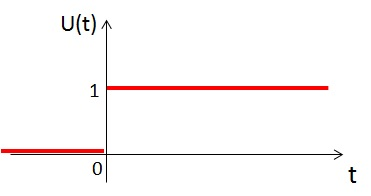
\includegraphics[scale=0.5]{images/Heaviside.jpg} 	
	\end{minipage}
	%\vspace{0.5\baselineskip}
	 
	\begin{equation}\label{Heaviside}
	u(t-t_{0}) = \left \{
	\begin{array}{l l}
	1  & si~t>t_{0} \\
	0   & sinon \\
	\end{array}
	\right .	 	
	\end{equation}
	
	
	Cette fonction peut être utilisée pour représenter n'importe quelle autre fonction avec une allure en marches d'escalier, comme l'illustre l'exemple présenté sur la figure \ref{Fig:Utilisation_Heaviside}. A partir de trois fonctions de Heaviside dont les instants d'apparition de l'échelon sont décalés, il est possible de générer une forme d'onde plus complexe.
	\begin{figure}[h!]
		\centering
		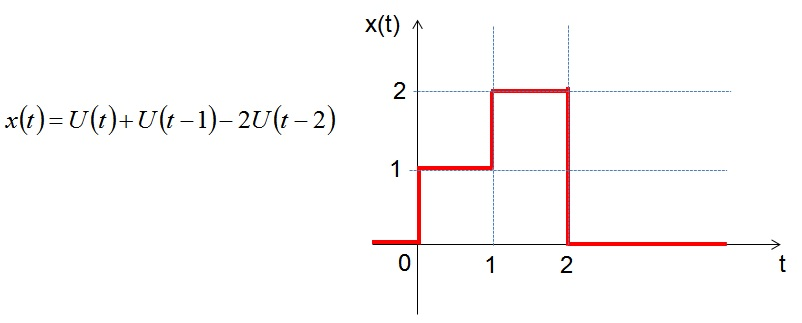
\includegraphics[scale=0.5]{images/Utilisation_Heaviside.jpg} 
		\caption{Exemple d'utilisation de la fonction de Heaviside pour bâtir une fonction plus complexe}	
		\label{Fig:Utilisation_Heaviside}
	\end{figure}
	
	La fonction de Heavisde peut servir de base pour générer d'autres fonctions, par intégration ou différenciation. Par exemple, en l'intégrant une fois, on obtient la fonction rampe. Si on l'intègre n fois, on peut obtient des fonctions présentant une croissance polynomiale en fonction du temps (\ref{integration_Heaviside}). 
	\begin{equation}\label{integration_Heaviside}
	u^{(-n)}(t) = \frac{t^{n}}{n!} \cdot u(t)	 	
	\end{equation}	
	Le cas de la dérivation est plus complexe car elle entraine l'apparition d'une discontinuité. En effet, la dérivée de la fonction de Heaviside devient infinie en $t_{0}$. Cet écueil ne peut se traiter qu'en utilisant la théorie des distributions, qui va permettre de définir l'impulsion de Dirac.
	
	\subsubsection{Impulsion ou distribution de Dirac}
	
	L'impulsion de Dirac se trouve en différenciant l'échelon unitaire (\ref{Dirac}). On
	voit immédiatement apparaître un problème : la dérivée est nulle partout, sauf là
	où l'échelon présente une discontinuité. Sa dérivée devient infinie.
	L'impulsion de Dirac n'est pas une fonction au sens classique, mais une
	distribution. Le bus de cette partie n'est pas de faire une présentation exhaustive de la théorie des distributions, mais de donner du sens à cette impulsion de Dirac, de décrire comment l'utiliser convenablement et de montrer son intérêt pour l'études des systèmes et des signaux. 

	
	\begin{minipage}[l]{0.45\linewidth}
			Il est possible de donner une justification physique à l'impulsion de Dirac, comme illustrée sur la figure ci-contre. On considère une fonction échelon avec un temps de transition finie $\tau$. En dérivant cette fonction, on obtient une fonction décrivant une impulsion brève de durée $\tau$. L'aire de cette fonction, associée à son énergie, est égale à 1. Au fur et à mesure que la durée $\tau$ décroit, l'amplitude de cette impulsion croit, mais son aire reste unitaire (équation \ref{Dirac_aire}). Le passage à la limite montre que l'impulsion tend à devenir nulle partout, sauf à l'origine où l'amplitude deviendrait infinie. L'impulsion de Dirac est donc une abstraction mathématique permettant de définir une impulsion infiniment courte.	
	\end{minipage} \hfill
	\begin{minipage}[r]{0.55\linewidth}
		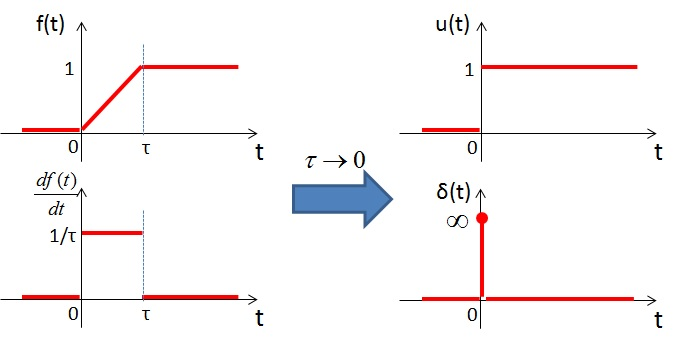
\includegraphics[scale=0.5]{images/generation_Dirac.jpg} 	
	\end{minipage}
	\vspace{0.5\baselineskip}
	
	\begin{equation}\label{Dirac_aire}
	\int_{\mathbb{R}}\delta (t)dt = 1 	
	\end{equation}
	\begin{equation}\label{Dirac_derive}
	\delta (t) = \frac{du(t)}{dt}	 	
	\end{equation}
	
	
	L'impulsion de Dirac est donc la dérivée de la fonction échelon unitaire (équation \ref{Dirac_derive}). La position de cette impulsion n'est pas forcément centré en 0. Elle peut être centrée n'importe où. De manière générale, on peut écrire que la distribution ou impulsion de Dirac est définie par l'équation \ref{Dirac}.
	\begin{equation}\label{Dirac}
	\delta (t-a) = \left \{
	\begin{array}{l}
	1~~~si~t = a \\
	0~~~sinon \\
	\end{array}
	\right . 	
	\end{equation}
	
	Quel peut être l'intérêt d'un tel objet mathématique, nul partout sauf en un point où il devient infini ? Il est certain qu'il ne peut être utilisé comme une fonction. Par contre, il peut servir à calculer une fonction indicatrice $I_{f}(\Delta)$ pour mesurer une caractéristique d'une fonction f, définie en $\mathbb{R}$, comme le montre l'équation \ref{Fonction_indicatrice}. La fonction f est localement intégrable et $\delta(t)$ sert de fonction test.
	\begin{equation}\label{Fonction_indicatrice}
	I_{f}(\delta)=\int_{\mathbb{R}}\delta(t-t_0)f(t)dt
	\end{equation}
	
	A l'intérieur de l'intégrale, la distribution de Dirac prend tout son sens. Elle va permettre de mesure la fonction f au point $t = t_0$. En effet, à l'intérieur de l'intégrale, en multipliant l'impulsion avec la fonction f et en l'intégrant sur un intervalle dt infiniment court, on prélève la valeur de la fonction f au point $t = t_0$. On appelle cette propriété la propriété d'échantillonnage, donnée par \ref{Dirac_echantillonage_1}. Celle-ci présente un très gand intérêt dans l'étude des signaux.
	
	\begin{equation}\label{Dirac_echantillonage_1}
	\int_{-\infty}^{+\infty} \delta (t) \cdot f(t) \deriv t = f(0) 	 
	\end{equation}
	\begin{equation}\label{Dirac_echantillonage_2} 	
	\int_{-\infty}^{+\infty} \delta (t-t_{0}) \cdot f(t) \deriv t = f(t_{0}) 
	\end{equation}
	
	Précisons-le à nouveau : l'utilisation de l'impulsion de Dirac n'a de sens qu'à l'intérieur d'une intégrale. Ce n'est pas une fonction classique au sens du terme mais une distribution, qui n'a pour but que de modéliser la mesure ou l'échantillonnage d'une fonction en un point. L'usage pratique montre qu'on trouve souvent l'impulsion de Dirac utilisée à l'extérieur de toute intégrale, comme une fonction mathématique classique. C'est bien entendu une écriture abusive et potentiellement source d'erreur. Cependant, ce type d'écriture permet parfois une simplification de l'écriture des calculs, qui est toléré si l'impulsion de Dirac est correctement employée dans une intégrale. Il est courant de représenter sur un graphique l'impulsion de Dirac, au même titre qu'une fonction. Techniquement, c'est impossible car l'amplitude de l'impulsion de Dirac devient infinie. Par convention, on la représente sous la forme d'un trait, terminé par une flèche, avec à proximité une valeur placée entre parenthèse indiquant l'aire du Dirac. La figure \ref{Fig:representation_Dirac} illustre cette représentation, avec l'affichage de l'impulsion $2\delta(t-1)$. L'impulsion est centrée en t = 1 et son aire est égale à 2. Sur ce graphe, on a superposé l'impulsion de Dirac avec le tracé d'une fonction f quelconque. L'utilisation de l'impulsion à l'intérieur de l'intégrale \ref{Dirac_echantillonage_2} permet d'extraire la valeur de f au point t = 1.
	
	
	
	\begin{figure}[h!]
		\centering
		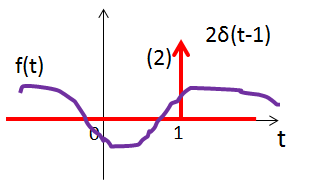
\includegraphics[scale=0.6]{images/representation_Dirac.png}
		\caption{Représentation graphique conventionnelle d'une impulsion de Dirac}	
		\label{Fig:representation_Dirac} 
	\end{figure}
	
	\vspace{1\baselineskip}
	Revenons au problème initial de sélection de familles d'excitation inchangées par l'effet d'un système LTI. On peut remarquer que cette propriété est aussi vérifiée avec la famille d'excitation impulsionnelle. L'action d'un opérateur proportionnel, intégrateur ou dérivée appliquée à une fonction de cette famille donnera une nouvelle fonction appartenant aussi à cette famille. De plus, on comprend intuitivement l'intérêt de l'impulsion de Dirac pour déterminer la réponse temporelle d'un système à n'importe quelle excitation. De par sa propriété d'échantillonnage, chaque point d'une excitation peut être modélisée, à la limite, par une impulsion de Dirac. L'excitation complète peut donc être modélisée comme la superposition d'un nombre infini d'impulsions de Dirac. Si on sait comment le système réagit à une impulsion de Dirac, la réponse à l'excitation sera la superposition des réponses à toutes les impulsions de Dirac, puisque le système est linéaire.
	
	\vspace{1\baselineskip}
	
	
	\section{Les différents types de réponse caractérisant les systèmes LTI}
	Maintenant que nous avons défini deux familles d'excitation adaptées à l'étude des systèmes LTI, nous pouvons définir plusieurs types de réponse qui nous aideront à analyser les propriétés de ces systèmes.
		
	
	\subsection{Réponse impulsionnelle}
	Elle correspond à la réponse d'un système excité par une impulsion de Dirac, que l'on note h(t). Même si l'amplitude de cette impulsion est infinie, son énergie vaut 1. Au lieu de représenter cette valeur infinie, nous utiliserons la valeur de 1. N'oublions pas qu'il ne s'agit pas d'une fonction mais d'une distribution, qui n'a du sens qu'à l'intérieur d'une intégrale.
	\begin{equation}\label{key}
	si~x(t)=\delta (t)~\rightarrow ~y_{f}(t)=h(t)
	\end{equation}
	Quel que soit le système LTI considéré, puisque l'excitation devient nulle pour t > 0, on retrouve le calcul de la réponse naturelle. L'application de l'impulsion en t=0 ne fait que changer les conditions initiales.
	
	\begin{equation}\label{}
	si~x(t)=\delta (t)~\rightarrow ~y_{f}(t) = y_{0}(t)	 	
	\end{equation}
	
	
	
	\vspace{1\baselineskip}
	La réponse impulsionnelle va nous fournir un moyen de calculer la
	réponse d'un système LTI à n'importe quelle excitation, en effectuant
	les calculs uniquement dans le domaine temporel. C'est ce que nous
	allons démontrer. Tout signal peut être vu comme la superposition d'un nombre infini de points, pouvant être modélisés par des impulsions de Dirac, pondérées et décalées dans le temps. Comme le montre
	la figure \ref{Fig:Approx_excitation_Dirac}, une excitation quelconque x(t) peut être
	approximée par une suite de rectangles adjacents, de largeur $ \Delta \tau $, que
	l'on peut remplacer par des impulsions de Dirac équivalentes de même
	surface. Ainsi, elles transportent la même énergie. Si la largeur $ \Delta \tau $
	tend vers zéro, cette approximation devient de plus en plus juste. Dans
	l'exemple considéré, on suppose que x(t) = 0 pour t \textless{} 0 par
	souci de lisibilité. Le même raisonnement resterait juste avec x(t) non
	nul pour t \textless{} 0. L'excitation peut alors s'approximer par :
	
	
	\begin{equation*}\label{}
	\sum_{n=-\infty}^{+\infty}x(n\Delta \tau) \cdot	\Delta \tau \cdot \delta (t-n\Delta \tau)	
	\end{equation*}
	
	\begin{figure}[h!]
		\centering
		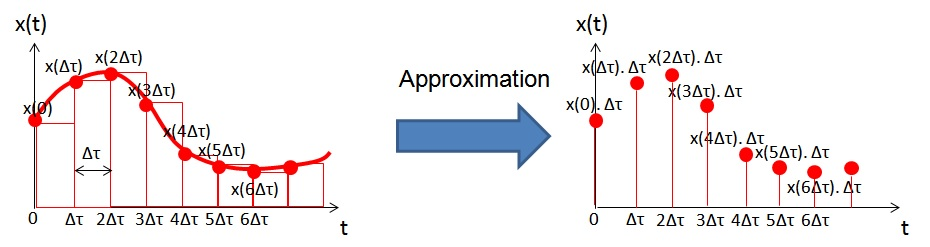
\includegraphics[scale=0.5]{images/Approx_excitation_Dirac.jpg} 
		\caption{Excitation quelconque x(t) approximée par une suite d'impulsion de Dirac}	
		\label{Fig:Approx_excitation_Dirac}
	\end{figure}
	Supposons que cette excitation attaque l'entrée d'un système LTI dont la réponse impulsionnelle h(t) est connue (Fig. \ref{Fig:reponse_impuls_illustration}). Par souci de lisibilité, on suppose aussi que h(t) = 0 pour t < 0.
	\begin{figure}[h!]
		\centering
		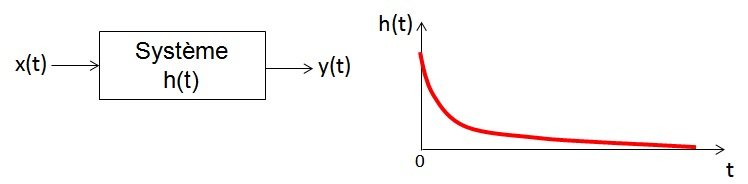
\includegraphics[scale=0.5]{images/reponse_impuls_illustration.jpg} 
		\caption{Réponse impulsionnelle d'un système}	
		\label{Fig:reponse_impuls_illustration}
	\end{figure}	
	
	Chaque impulsion élémentaire composant x(t) et apparaissant à l'instant
	$ k \times \Delta \tau $ contribue à la réponse en sortie, comme l'illustre la figure \ref{Fig:illustration_reponse_impuls_2}. Chacune d'entre elles produit une réponse égale à la réponse impulsionnelle du système, mais :
	
	\begin{itemize}
		\item pondérée par l'amplitude de l'excitation d'entrée à l'instant $ k \times \Delta \tau $
	
		\item décalée dans le temps de $ k \times \Delta \tau $~
	\end{itemize}
	\begin{figure}[h!]
		\centering
		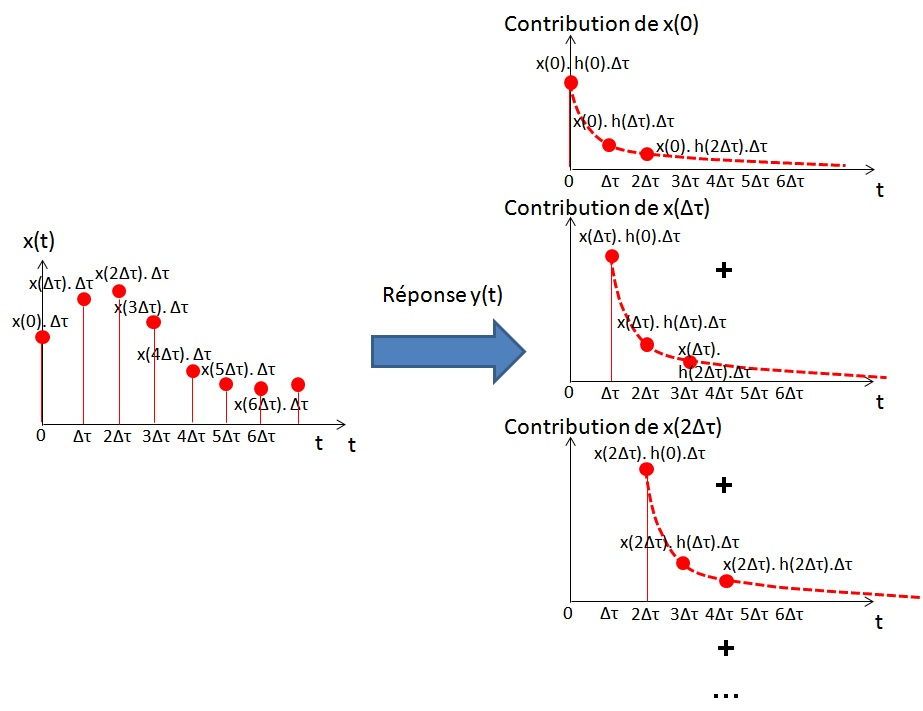
\includegraphics[scale=0.5]{images/illustration_reponse_impuls.jpg} 
	\end{figure}
	\begin{figure}[h!]
		\centering
		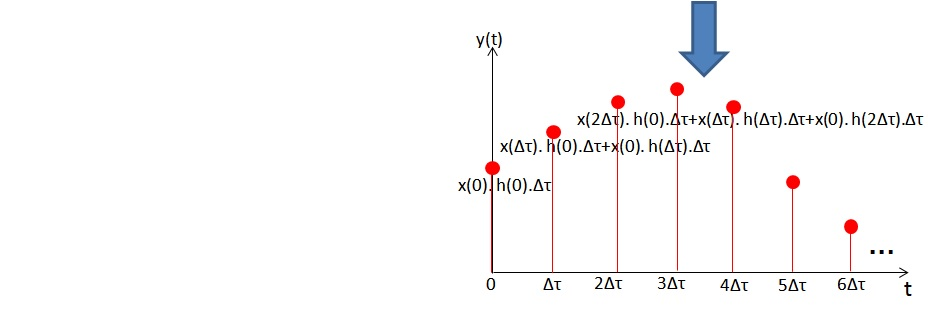
\includegraphics[scale=0.6]{images/illustration_reponse_impuls_2.jpg}
		\caption{Construction de la réponse impulsionnelle}	
		\label{Fig:illustration_reponse_impuls_2} 
	\end{figure}

	La réponse globale du système est obtenue en sommant l'ensemble des contributions de chaque impulsion élémentaire formant l'excitation. Elle peut alors s'approximer par : 
	\begin{equation*}\label{key}
	\sum_{n=-\infty}^{+\infty} x(n\Delta \tau) \cdot \Delta \tau \cdot h(t-n\Delta \tau)
	\end{equation*}
	
	En faisant tendre $ \Delta \tau $ vers zéro, cette somme converge vers une intégrale
	donnée par la relation ci-dessous. Ce calcul intégral particulier,
	faisant intervenir le produit de deux fonctions dont les indices $\tau $ et
	t-$\tau $ sont balayés dans des directions opposées, porte un nom : le produit
	de convolution. Cette opération est symbolisée par le signe *.
	\begin{equation}\label{Demo_produit_convolution}
	y(t) = \lim_{\Delta t \to 0} \sum_{n=-\infty}^{+\infty} x(n\Delta t) \cdot \Delta t \cdot h(t-n\Delta t) = \int_{-\infty}^{+\infty} x(\tau) \cdot h(t-\tau) \deriv \tau = x*h(t)
	\end{equation}
	
	Cette relation basée sur le produit de convolution fournit donc un outil de calcul de la réponse du système directement dans le domaine temporel. Cependant, c'est un calcul complexe, passant par une opération longue et fastidieuse si elle est effectuée à la main. Nous y reviendrons au chapitre 7, qui sera consacré au calcul des réponses des systèmes LTI directement dans le domaine temporel. Cependant, avant d'aborder ce point, nous allons d'abord considérer le cas d'une excitation exponentielle complexe pour dériver le concept de fonction de transfert défini dans le domaine fréquentiel. Nous verrons que dans ce domaine, le calcul de la réponse du système est beaucoup plus aisée !
	
	\subsubsection{Condition pour garantir la causalité}
	Un système est causal si sa réponse ne dépend que des états passés et présents. A partir de la réponse impulsionnelle, on peut en déduire une condition : il faut que h(t) = 0 pour t < 0. Les systèmes causaux sont les seuls à être physiquement réalisables. Le calcul de la réponse d'un système causal à partir de sa réponse impulsionnelle peut s'écrire :
	\begin{equation}\label{}
	y(t) = \int_{0}^{+ \infty} x(\tau) \cdot h(t-\tau)d\tau = x*h(t)
	\end{equation}
	\vspace{1\baselineskip}	
	
	\subsection{Réponse indicielle}
	Elle correspond à la réponse d'un système excité par une fonction de Heavisde. On la note a(t).
	\begin{equation}\label{key}
	si~x(t)=u(t)~\rightarrow ~y_{f}(t)=a(t)
	\end{equation}

	\vspace{0.5\baselineskip}
	
	\textbf{\underline{Autre manière de déterminer la réponse impulsionnelle}}
	
	Sans démonstration, on peut affirmer que si on différencie l'excitation, on peut déterminer la nouvelle réponse en différenciant la réponse à l'excitation initiale : si $y(t) = L[x(t)]$ alors $\frac{dy}{dt} = L[\frac{dx}{dt}] $.
	Ainsi, puisque l'impulsion de Dirac est la dérivée de l'échelon unitaire, si on connait la réponse indicielle, on peut retrouver la réponse impulsionnelle en dérivant la réponse indicielle.
	
	\begin{equation}\label{key}
	\delta(t)=\frac{da(t)}{dt}
	\end{equation}
	
	\vspace{0.5\baselineskip}
	
	
	\subsection{Réponse à une exponentielle complexe - Fonction de transfert}
	On considère une excitation exponentielle complexe. La réponse forcée a donc la même forme que l'excitation, et présente la même fréquence complexe. La seule inconnue est le phaseur $\hat{Y}$ de la réponse. Soit l'excitation $ x(t) = Re[\hat{X} \cdot e^{pt}]$ et la réponse $ y_{f}(t) = Re[\hat{Y} \cdot e^{pt}]$ pour t > 0. Si on reprend l'équation différentielle ordinaire générale d'un système LTI donnée par \ref{equation_generale_LTI}, on peut écrire la relation suivante.
	
	\begin{equation*}\label{}
	\sum a_{i} \cdot Re[p^{i} \cdot \hat{Y} \cdot exp(pt)] = \sum b_{i} \cdot Re[p^{j} \cdot \hat{X} \cdot exp(pt)]
	\end{equation*}
	\begin{equation*}\label{}
	\sum a_{i} \cdot Re[p^{i} \cdot \hat{Y}] = \sum b_{i} \cdot Re[p^{j} \cdot \hat{X}]
	\end{equation*}
	\begin{equation*}\label{}
	\hat{Y} \cdot \sum a_{i} \cdot Re[p^{i}] = \hat{X} \cdot \sum b_{i} \cdot Re[p^{j}]
	\end{equation*}
	
	On peut donc facilement déterminer le phaseur $\hat{Y}$ associée à la réponse, c'est-à-dire le module et le déphasage de la réponse. 
	On peut alors caractériser l'effet du système à une excitation exponentielle complexe quelconque sous une forme appelée fonction de transfert, définie comme le rapport entre les phaseurs de réponse et d'excitation, et défini pour toutes les fréquences complexes. 
	\begin{equation}\label{Def_fonction_tranfert}
	H(p) = \frac{Y}{X} (p) = \frac{\hat Y}{\hat X} (p)= \frac{\sum a_{i} \cdot Re[p^{i}]}{\sum b_{i} \cdot Re[p^{j}]}=G\frac{\prod_{i=1}^{M} (p-p_{i})}{\prod_{j=1}^{N} (p-p_{j})}
	\end{equation}
	De manière générale, l'équation \ref{Def_fonction_tranfert} peut s'écrire comme une fraction rationnelle entre deux polynômes, où G est un terme constant. Les N racines du dénominateur sont les pôles de la fonction de transfert et les M racines du numérateur sont appelées les zéros de la fonction de transfert. Comme leur nom l'indique, ils annulent la fonction de transfert lorsque la fréquence $p=p_{j}$. Les pôles sont les mêmes que ceux identifiés dans la réponse naturelle ! Ils ont un rôle prépondérant sur la stabilité du système et la nature de la réponse. Les outils permettant d'étudier l'influence des pôles et des zéros sur la réponse d'un système sortent du cadre de ce cours et seront abordés dans les cours d'automatique.\\
	
	Avec une excitation exponentielle complexe, l'action du système LTI peut donc se résumer à la multiplication de l'excitation par la fonction de transfert.
	On peut souligner la facilité de la méthode. Une fois la fonction de transfert connue à une fréquence complexe donnée, la réponse forcée à une exponentielle complexe de même fréquence est trouvée en multipliant le phaseur d'entrée par la fonction de transfert (\ref{Relation_Entree_Sortie_Fonction_Transfert}).
	\begin{equation}\label{Relation_Entree_Sortie_Fonction_Transfert}
	\hat{Y}(p) = H(p)\cdot \hat{X}(p)=|H(p)||X(p)|e^{j(arg(H(p))+arg(\hat{X}(p)))}	
	\end{equation}
	
	\vspace{1\baselineskip}
	
	
	\textbf{\underline{Réponse en régime permanent :} }
	
	Dans le cas général, l'excitation est complexe. Le cas particulier où $\sigma$ = 0 correspond au cas d'une excitation dite monochromatique ou harmonique. On parlera alors de réponse en fréquence. Il correspond aussi au cas du régime permanent avec $\sigma$ < 0, c'est-à-dire que t devient suffisamment grand pour que l'influence du terme $e^{\sigma t}$ devienne négligeable. 
	La réponse du système se trouve facilement en remplaçant la fréquence complexe p par $j\omega$. En considérant une excitation cosinusoïdale d'amplitude égale à X et de phase $\Phi_{x}$, la réponse du système est donnée par la relation suivante.
	
	\begin{equation}\label{calcul_reponse_fonction_transfert}
	y(t) = Re[|H(\omega)|X\cdot e^{j(\omega t+arg(H(p))+\Phi_{x})}] =|H(\omega)|X\cdot cos(\omega t+arg(H(p))+\Phi_{x})
	\end{equation}
	
	La réponse est une grandeur complexe. Le module de la réponse en fréquence est le gain en amplitude de la fonction de transfert du système ou du filtre. Le déphasage du signal en sortie du filtre par rapport au signal d'entrée est l'argument de la fonction de transfert. Le module et la phase sont des fonctions de la pulsation $\omega$.
	
	
	\subsubsection{Exemple}
	
	\begin{minipage}[l]{0.7\linewidth}
		On reprend l'exemple du circuit RC abordé dans la partie IV.4. On considère toujours que le condensateur est chargé initialement en t = 0, avec une tension à ses bornes notée $U_C0$. Le circuit est excité par un signal délivrant une excitation exponentielle complexe $U_{E}(t)=Xe^{pt}$ avec t > 0 et X l'amplitude complexe. La réponse du circuit correspond à la tension mesurée aux bornes de la résistance R ou tension de sortie. Déterminez la fonction de transfert de ce circuit. Indiquez quels sont les pôles et les zéros. Quelle est la réponse à un signal cosinuoïdal, d'amplitude unitaire et de phase nulle ?	
	\end{minipage} \hfill
	\begin{minipage}[r]{0.4\linewidth}
		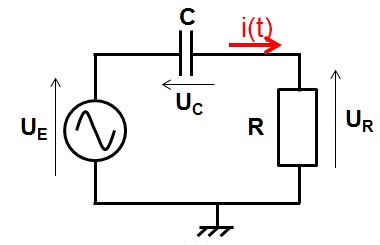
\includegraphics[scale=0.5]{images/circuit_RC_reponse_forcee.jpg} 	
	\end{minipage}
	\vspace{0.5\baselineskip}

	La réponse du circuit $U_{R}$ est la superposition de la réponse naturelle $U_{R0}$ et de la réponse forcée $U_{Rf}$. La réponse naturelle est liée à la présence d'une condition initiale : ici, le stockage d'une charge dans le condensateur à t=0. Sans charge initialement stockée, la réponse naturelle aurait été nulle. Nous avions établi la réponse naturelle de ce circuit en terme de courant. Nous pouvons aisément l'adapter pour la donner en terme de tension de sortie.
	\begin{equation*}\label{}
	U_{R0}(t)=Ri_{0}(t)=U_{C0}exp(-\frac{t}{RC})~,~~t>0
	\end{equation*}
	La réponse forcée est provoquée par l'excitation du circuit en t > 0, indépendamment de la présence d'une condition initiale. Commençons par établir une équation différentielle reliant la tension de sortie $U_{Rf}$ et l'excitation $U_{E}(t)$. On utilise la loi des mailles. Après une dérivation, on obtient l'équation \ref{equa_diff_reponse_forcee_RC}.
	\begin{equation*}\label{}
	U_{E}(t)=U_{C}(t)+U_{R}(t) ~ \Rightarrow ~ U_{E}(t)=\frac{1}{C}\int i(t) \deriv t+U_{R}(t)~ \Rightarrow ~U_{E}(t)=\frac{1}{RC}\int U_{R}(t) \deriv t+U_{R}(t)
	\end{equation*} 
	\begin{equation}\label{equa_diff_reponse_forcee_RC}
	\frac{dU_{E}}{dt}=\frac{U_{R}}{RC}+\frac{dU_{R}}{dt}
	\end{equation}
	L'excitation étant de type exponentielle complexe et le circuit linéaire, la réponse est aussi de type exponentielle complexe. Elle s'écrit : $U_{Rf}(t)=Ye^{pt}$. Replaçons les termes $U_{E}$ et $U_{R}$ par leurs expressions respectives dans \ref{equa_diff_reponse_forcee_RC} et exprimons le rapport entre ces deux grandeurs pour obtenir la fonction de transfert H(p) de ce circuit (équation \ref{TF_RC_forcee}).
	\begin{equation*}
	pXe^{pt}=\frac{1}{RC} Ye^{pt}+pYe^{pt} ~\Rightarrow~pU_{E}(t)=\frac{1}{RC}U_{Rf}(t)+pU_{Rf}(t)
	\end{equation*}
	\begin{equation}\label{TF_RC_forcee}
	H(p)=\frac{U_{Rf}}{U_{E}}(p)=\frac{p}{p+\frac{1}{RC}}=\frac{p}{p+\omega_{0}}~,~\omega_{0}=\frac{1}{RC}
	\end{equation}

	La fonction de transfert du système présente un zéro nul et un seul pôle $p_{0}$, qui est exactement le même que celui identifié dans l'analyse de la réponse naturelle. Ce n'est pas une surprise car les pôles agissent sur la stabilité, qui est une caractéristique intrinsèque du système indépendante de l'excitation. Le pôle étant purement réel et négatif, on peut conclure que le système sera stable.
		
	Calculons maintenant la réponse forcée à un signal cosinusoïdale, en utilisant \ref{calcul_reponse_fonction_transfert}. Le système n'agit que sur l'amplitude et la phase de l'excitation. Il est donc intéressant d'exprimer la fonction de transfert sous la forme de son module et son déphasage. En considérant $p=j\omega$, celles-ci sont :
	\begin{equation*}
	|H(\omega)|=\frac{\omega}{\sqrt{\omega^{2}+\omega_{0}^{2}}}~~~et~~Arg(H(\omega))=\frac{\pi}{2}-atan(\frac{\omega}{\omega_{0}})
	\end{equation*}
	\begin{equation*}
	\Rightarrow~U_{Rf}(t)=|H(\omega)|cos(\omega t+Arg(H(\omega)))
	\end{equation*}
	La réponse étant la superposition des réponses naturelles et forcées, celle-ci s'écrit :
	\begin{equation*}
	\Rightarrow~U_{R}(t)=U_{Rf}(t)+U_{R0}(t)=|H(\omega)|cos(\omega t+Arg(H(\omega)))+U_{C0}exp(-\frac{t}{RC})
	\end{equation*}
	
	\vspace{1\baselineskip}

	\subsection{Calcul de la réponse d'un système dans le domaine temporel ou fréquentiel ?}
	
	Nous venons de décrire deux manières de calculer l'effet d'un système LTI, selon que l'on considère une excitation impulsionnelle ou exponentielle complexe. Dans le premier cas, la réponse est déterminée directement dans le domaine temporel à l'aide de l'équation \ref{Demo_produit_convolution} et de la réponse impulsionnelle, à l'aide d'un produit de convolution. Dans le second cas, la réponse est déterminée dans le domaine fréquentiel à l'aide de l'équation \ref{calcul_reponse_fonction_transfert} et de la fonction de transfert.	
	Bien qu'il semble plus naturel de faire le calcul de la réponse directement dans le domaine temporel, nous avons montré que le calcul dans le domaine fréquentiel était beaucoup plus évident. Il se résume à une simple multiplication de l'excitation par la fonction de transfert. 
	Cependant, comme il s'agit du même système, il y a nécessairement un lien entre la réponse impulsionnelle et la fonction de transfert. C'est ce que nous verrons dans les prochains chapitres, où nous aborderons les questions de transformée de Laplace, puis de Fourier. Nous allons ainsi mettre en évidence des transformations mathématiques, permettant le passage d'une fonction du domaine temporel au domaine fréquentiel, et inversement.
	
	\vspace{1\baselineskip}	

	
	
	\section{Exercices}
	
	\subsubsection{Exercice 1} 
	Soient les systèmes dont le comportement temporel est défini par les équations suivantes. Indiquez si ces systèmes sont linéaires, à temps invariant et causaux ?
	
	a. $y(t) = x(t)+4\frac{dy}{dt}$ 
	
	b. $y(t) = 2x(t)+2$ 
	
	c. $y(t)=e^{-t}x(t-2)^{2}$
	
	d. $y(t)=\frac{dx}{dt}+x(t+2)$
	
	\vspace{1\baselineskip}
	
	\subsubsection{Exercice 2} 
	1. On trace les réponses de deux systèmes LTI ((a) et (b)). Proposez une expression mathématique décrivant ces réponses.
	\begin{figure}[h!]
		\centering
		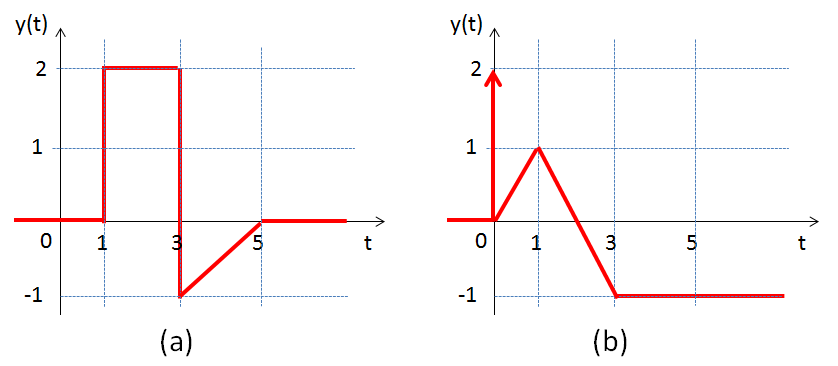
\includegraphics[scale=0.5]{images/Exo_2_2.jpg} 
	\end{figure} 

	
	2. Réécrivez sous la forme d'une fonction à valeurs réelles les fonctions suivantes et esquissez leur forme temporelle (pour t >0) :
	
	a. $x(t) = (1+j)e^{j\cdot 10t}$ 
	
	b. $y(t) = e^{(-2+j)t}\cdot u(t-2)$ 
	
	c. $z(t) = e^{(-1+2j)t}+e^{(-1-2j)t}$
	
	\vspace{1\baselineskip} 
	
	
	
	\subsubsection{Exercice 3}
	
	On dispose de la réponse indicielle d'un système linéaire, qui est esquissée ci-dessous. Elle a une forme exponentielle croissante.\\
	
	\begin{figure}[h!]
		\centering
		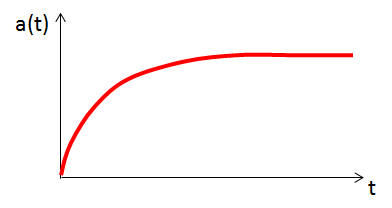
\includegraphics[scale=0.5]{images/Exo_2_3.png} 
	\end{figure} 
	
	Esquissez les réponses de ce système dans les cas suivants :\\
	
	a. l'excitation $e(t)=u(t)-u(t-1)$\\
	
	b. l'excitation $e(t)=t(u(t)-u(t-2))$\\
	
	c. l'excitation est la dérivée de celle utilisée pour obtenir la réponse indicielle.\\
	
	\subsubsection{Exercice 4}
	
	On excite un système linéaire à l'aide du signal suivant : $e(t)=e^{j2\pi t}$. La réponse obtenue, notée y(t), est égale à $y(t)=\frac{1}{2}e^{j(2\pi t+\frac{\pi}{3})}$.\\
	
	a. Réécrire la réponse sous la forme $y(t)=Acos(\omega t + \phi)$ et $y(t)=Bcos(\omega t)+Csin(\omega t)$, en précisant les valeurs de A, B, C et $\phi$.\\
	
	b. Donnez l'expression de la réponse du système lorsqu'il est excité par le signal ci-dessous.
	
	\begin{figure}[h!]
		\centering
		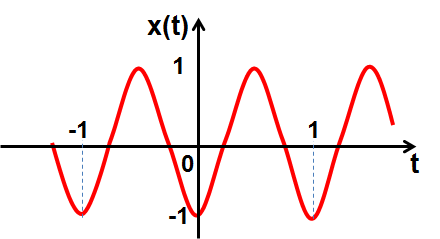
\includegraphics[scale=0.5]{images/Exo_2_4.png} 
	\end{figure} 
	
	c. Calculez la réponse du système à l'excitation suivante : $x(t)=\frac{3\sqrt{3}}{2}cos(2\pi t)+\frac{1}{2}sin(2\pi t)$.\\
	
	
	
	\subsubsection{Exercice 5 - Réponse indicielle d'un circuit RC}
	
	On reprend le circuit RC dont on a étudié la réponse dans la partie VI.3. On considère deux cas : celui où le condensateur est déchargé initialement, puis celui où il est chargé. 
	
	a. Calculez la réponse naturelle du circuit lorsque le condensateur est initialement chargé.
	
	b. En déduire la réponse impulsionnelle du circuit.
	
	c. Calculez la réponse lorsque le circuit est soumis à un échelon de Heaviside d'amplitude E, dans les deux cas (charge initiale absente ou présente).
	
	d. En déduire la réponse indicielle du circuit.
	
	\vspace{1\baselineskip}	
	

	
	\subsubsection{Exercice 6}
	
	On considère les deux circuits électriques ci-dessous. Pour le circuit (a), la tension initiale (t=0) aux bornes du condensateur C est notée $U_{C0}$. Pour le circuit (b), un courant noté $I_L0$ traverse la bobine L. La sortie de ces deux circuits est la tension $U_{S}$.
	
	\begin{figure}[h!]
		\centering
		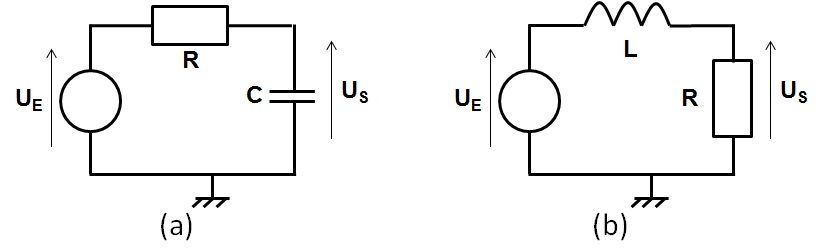
\includegraphics[scale=0.5]{images/Exo_2_4.jpg} 
	\end{figure} 
	
	a. Déterminez les fréquences et les réponses naturelles de ces deux circuits. Quels sont les ordres de ces deux systèmes ? 
	
	b. On excite ces deux systèmes à l'aide d'un échelon de Heaviside d'amplitude notée E. Déterminez la réponse indicielle de ces deux circuits. 
	
	c. Déterminez les fonctions de transfert de ces deux circuits.
	
	\vspace{1\baselineskip}
	
	\subsubsection{Exercice 7 - Fonction de transfert d'un circuit résonant}
	
	On reprend le circuit RLC présenté dans la partie IV.4. Celui-ci est excité par un générateur de courant I, comme le montre la figure ci-dessous. On s'intéresse à la tension U aux bornes de ce circuit. On considère que la résistance R est grande et $R>>\sqrt{\frac{L}{C}}$.
 	 	
 	\begin{figure}[h!]
 		\centering
 		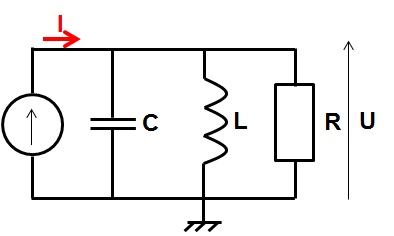
\includegraphics[scale=0.5]{images/Exo_2_5.jpg} 
 	\end{figure} 
 
 	a. Déterminez la fonction de transfert de ce circuit. La mettre sous la forme $\frac{Gp}{p^2+2\alpha p+\omega_{0}^{2}}$.\\
 	
 	b. Précisez l'unité de la fonction de transfert. \\
 	
 	c. Ce circuit est-il stable ?\\
 	
 	d. On considère maintenant que le terme $\alpha$ est négligeable et une excitation cosinusoïdale du circuit. Y a t-il une fréquence particulière où la réponse présente un maximum ? Si oui, laquelle ? \\
 	
 	e. Donnez l'expression de la réponse temporelle du circuit en régime permanent.\\
	
	\vspace{1\baselineskip}
	
	\subsubsection{Exercice 8}
	
	On considère le système dont le fonctionnement est décrit par le schéma-bloc ci-dessous. Celui-ci transforme un signal d'entrée e(t) et délivre en sortie un signal s(t). 
	
	\begin{figure}[h!]
		\centering
		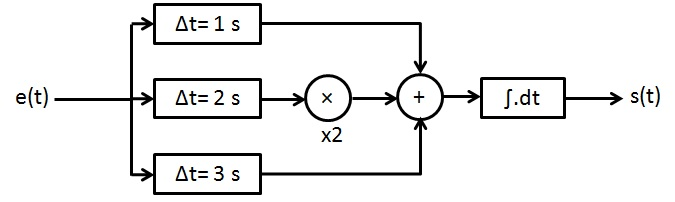
\includegraphics[scale=0.5]{images/Exo_2_6.jpg} 
	\end{figure}
	
	a. Le système est-il linéaire, à temps invariant, causal ?
	
	b. Ecrire l'équation différentielle générale de ce système.
	
	c. Déterminez l'expression de la réponse impulsionnelle h(t) du système. Esquissez l'allure temporelle de la réponse impulsionnelle. 
	
	d. Déterminez l'expression de la fonction de transfert H(p) du système. Précisez les pôles de la fonction de transfert. Que concluez-vous sur sa stabilité ?
	

	



%%% Pour compiler avec emacs
%%% Local Variables:
%%% mode: latex
%%% TeX-master: "main"
%%% End:
